% (fold)
% Template: LaTeX file for ICMC 2010 papers, with hyper-references
%
% derived from the DAFx-06 templates
% derived from the ICMC 2009 templates by Steve Beck
%
% 1) Please compile using latex or pdflatex.
% 2) Please use figures in vectorial format (.pdf); .png or .jpg are working otherwise 
% 3) Please use the "papertitle" and "pdfauthor" commands defined below

%------------------------------------------------------------------------------------------
\documentclass[twoside,10pt]{article}
\usepackage{icmc2010,amssymb,amsmath} 
%\setcounter{page}{1}

\usepackage{mathptmx} 

%____________________________________________________________
%  !  !  !  !  !  !  !  !  !  !  !  ! user defined variables  !  !  !  !  !  !  !  !  !  !  !  !  !  !
%==== set the title ====
\def\papertitle{A Flexible and Dynamic C++ Framework and Library for Digital Audio Signal Processing}
%\def\papertitle{}	%-- should be empty for the submission anyway!

%==== 1st submission: author name and affiliation are empty for anonymous submission ====
\def\paperauthorA{} 
\affiliation{}{}


%==== final submission: author name and affiliation ====
%---- uncomment 1 to 4 lines, for 1 to 4 authors
\def\paperauthorA{First Author}
\def\paperauthorB{Second Author}
\def\paperauthorC{Third Author}
\def\paperauthorD{Fourth Author}

%%---- set correspnding affiliation data for...
%%-- 1 author
%\affiliation{\paperauthorA}
%  {School\\ Department, City, Country \\ {\tt \href{mailto:email@domain.icmc}{email@domain.icmc}}}

%%-- 2 authors with same affiliation
%\affiliation{\paperauthorA, \paperauthorB}
%  {School\\ Department, City, Country \\ {\tt \href{mailto:email@domain.icmc}{email@domain.icmc}}}

%-- 2 authors with different affiliations
%\twoaffiliations{\paperauthorA}{School\\ Department}
%  {\paperauthorB}{Company\\ Address}

%%-- 3 authors with different affiliations
%\threeaffiliations{\paperauthorA}{School A\\ Department X}
%  {\paperauthorB}{Company\\ Address}
%  {\paperauthorC}{School B\\ Department Y}

%%-- 4 authors with different affiliations
%\fouraffiliations{\paperauthorA}{School A\\ Department X}
%  {\paperauthorB}{Company\\ Address}
%  {\paperauthorC}{School B\\ Department Y}
%  {\paperauthorD}{School C\\ Department Z}

%  ^  ^  ^  ^  ^  ^  ^  ^  ^  ^ user defined variables  ^  ^  ^  ^  ^  ^  ^  ^  ^  ^  ^  ^ 
%------------------------------------------------------------------------------------------

%%-- if using .ps or .eps figure files, they will be converted on the fly
%%-- RMK: for faster LaTeX runs, use it only once after adding new \includegraphics[]{} cmds
%\usepackage{epstopdf}	 

%---- the hyperref package must be last to properly work
\usepackage[pdftex,
       pdftitle={\papertitle},
	pdfauthor={\paperauthorA},
	colorlinks=false,bookmarksnumbered,pdfstartview=XYZ]{hyperref}
%\pdfcompresslevel=9
\usepackage[pdftex]{graphicx}	% for compatible graphics with hyperref
\usepackage[figure,table]{hypcap}	% corrects the hyper-anchor of figures/tables

% Stuff added by [tap]
\usepackage{hyperref}
\usepackage{url}
\usepackage{amsmath}
\usepackage{color}
\definecolor{black}{rgb}{0,0,0}
\hypersetup{colorlinks
,linkcolor=black
,filecolor=black
,urlcolor=black
,citecolor=black}
%reduces the space between the items in the itemize-environment 
\newenvironment{packed_item}{
\begin{itemize}
  \setlength{\itemsep}{1pt}
  \setlength{\parskip}{0pt}
  \setlength{\parsep}{0pt}
}{\end{itemize}}



\title{\papertitle}
% (end)

%------------------------------------------------------------------------------------------
\begin{document}

\DeclareGraphicsExtensions{.png,.jpg,.pdf} % used graphic file format for pdflatex
    
\maketitle

%%%%%%%%%%%%%%%%%%%%%%%%%%%%%%%%%%%%%%%%%%%%%%%%%%%%%%%%%%%%%%%%%%%%%%%%%%%%%%%%%%%%%%%%%%%

\begin{abstract}

This paper presents an object-oriented, reflective, light-weight application programming interface for C++, with an emphasis on real-time signal processing. It makes use of polymorphic typing, dynamic binding, and introspection to create a cross-platform environment pulling ideas from languages such as Smalltalk and Objective-C while remaining within the bounds of the portable and cross-platform C++ context.  The Jamoma Foundation and DSP Library provide a flexible framework and runtime environment, as well as an expanding collection of unit generators for synthesis, processing, and analysis.  This library has been used in both open source and commercial software projects over the past seven years.

\end{abstract}


%%%%%%%%%%%%%%%%%%%%%%%%%%%%%%%%%%%%%%%%%%%%%%%%%%%%%%%%%%%%%%%%%%%%%%%%%%%%%%%%%%%%%%%%%%%

\section{Introduction} % (fold)
\label{sec:introduction}

``The SMC Roadmap identifies two broad research challenges: (1) To design better sound objects and environments and (2) To understand, model, and improve human interaction with sound and music.'' \cite{serra:2007}  The Jamoma DSP library directly addresses the first task as means by which to address the second task.

% CHANGED: More interesting where we are now rather than how we got here, as suggested by Trond
%\subsection{History}
%
% Came out of Tap.Tools and Hipno development.  This was pre-Electrotap, so maybe the credit here should somehow go to 74Objects?
%


\subsection{Terminology}

It is useful to clarify our usage of various computer science jargon and terminology.  In \emph{object-oriented programming} functionality related to a set of data is treated as a unit.  These units, or objects, are created and then often passed using a reference or pointer to the memory in which the object's contents are stored.  These objects comprise \emph{methods} (functions) and \emph{attributes} (properties or data which represents state).

\emph{Polymorphism} is a means by which a programming language generalizes different types of functions or data using a common \emph{API}, or Application Programming Interface.  An example of a polymorphic data-type of the variety in which we are interested is a `var' in the Javascript language.  That is to say a data type which may be any data type internally (including an object or array), the details of which are not necessary in order to use or pass the data type amongst functions.

\emph{Introspection} refers to the ability to determine the characteristics of an object at runtime.  This means that when handed a pointer in C++, we can take the pointer and query for an object's name, its type or \emph{class}, the messages that it understands, the attributes it possesses, etc.  By extension, \emph{reflection} refers to the ability to then modify the behavior of an object at runtime.  In practical terms this means adding messages, changing attributes, and extending existing instances of objects as the software is executing and without stopping the software to re-compile the code.

Introspection and reflection are often implemented by making use of a \emph{dynamic binding model}.  Programming languages including C++ and Java link function and method calls when a program is compiled, known as static binding.  A dynamically bound model does not link these functions at compile-time, but instead waits until runtime to resolve the address of a method being called.  When a dynamic binding model is in use, calling methods is referred to as `sending messages' to objects.  Dynamic binding is the hallmark of languages such as Smalltalk, Objective-C, and Ruby.

Throughout the literature exists a confusing gaggle of terminology for classifying systems of objects.  These include \emph{framework}, \emph{library}, \emph{environment}, and \emph{toolkit}.  For the purposes of this paper, these will be defined as follows.  

\begin{packed_item}%\begin{itemize}
	\item unit generator : A class or object that implements a well-defined DSP task such as generating, analyzing, or processing audio data.
	\item library : a collection of pre-built, ready-to-use, unit generators
	\item toolkit	: a collection of functions, helpers, possibly with an API, for creating unit generators
	\item framework : 
	\item environment : au/vst/max/sc3/chuck
	\item runtime : 
\end{packed_item}%\end{itemize}


\subsection{Requirements}

The authors are involved in a number of divergent and parallel efforts requiring a both a framework for creating unit generators and a library of ready-to-go unit generators.  These efforts include both open-source and closed-source commercial applications targeting multiple platforms and environments.  To meet the manifold demands of these endeavors the following list of requirements must be met regarding how said framework must perform and behave.

\begin{packed_item}%\begin{itemize}
	\item liberal licensing for both open source and commercial end use
	\item cross-platform (Mac/Windows/Linux/Embedded Devices/Mobile Platforms)	
	\item effortless to wrap (integrate?) classes for use in different environments (Max/MSP, VST, AU, ChucK, Pd)
	\item user-extensible
	\item dynamically reconfigurable classes at runtime (object decoration, process routine switching)
	\item multichannel support
	\item reasonably efficient (i.e. frame-based audio processing)
	\item process methods must be able to adapt to varying input (frame sizes, channel configurations, etc.) on-the-fly
	\item must support 64-bit audio streams (future proof ?)
	\item be as thread-agnostic as possible (don't manage it, but take care of requisite protection, adaptable to various architectures)
	\item MVC-friendly (reconfigurable)
\end{packed_item}%\end{itemize}

Having met these technical requirements, the authors also deem an additional set of process requirements to be important.  These requirements are in adhering to contemporary philosophies for good coding practice, ensuring that it is pleasant to work with the code, to maintain it, to test it, and to distribute it.

\begin{packed_item}%\begin{itemize}
	\item expressive syntax, idioms, and conventions
	\item adhere to the DRY principle (Don't Reapeat Yourself): ``Every piece of knowledge must have a single, unambiguous, authoritative representation within a system''\cite{Hunt:1999}
	\item clear code % what do we mean by this?
	\item convention over configuration
	\item tag-based searching for class categorization and object instantiation
	\item integrated unit testing and benchmarking % TODO: reference
\end{packed_item}%\end{itemize}


% One list for efficiency to the computer
% One list for efficiency for the development process / programmers's workflow : Ruby : set out top make a program that would "make programmers happy"; "Ruby is simple in appearance, but is very complex inside, just like our human body" - Yukihiro “matz” Matsumoto

% (end)


%%%%%%%%%%%%%%%%%%%%%%%%%%%%%%%%%%%%%%%%%%%%%%%%%%%%%%%%%%%%%%%%%%%%%%%%%%%%%%%%%%%%%%%%%%%

\section{Prior Art} % (fold)

A myriad of existing libraries, toolkits, frameworks, and environments are available for digital signal processing.  To justify the effort of creating a new framework the merits of the extant members in this field should be considered, particularly with regard to our previously stated requirements.


\subsection{Choice of Language} % (fold)

An immediate winnowing of the field of contenders can be accomplished by discussing the choice of programming language.  There are popular and well structured DSP libraries for Java\cite{Guillemard:2005, Burk:1998} and Objective-C\cite{Jaffe:1989,Jaffe:1991}, for example, but these languages also carry restrictions and baggage.  Java is not installed on Windows systems by default and is not available in the context of many embedded devices.  Objective-C is available on Windows only through the clumsy and inadequate GnuStep\footnote{\url{http://www.gnustep.org/}} project\footnote{For example, one cannot natively compile using Microsoft's MSVC compiler.} and also is not available in the context of many embedded or mobile devices\footnote{The authors also look upon Apple's corporate control of the Objective-C language and runtime with some degree of skepticism, as compared to the open consortium that is mediating the C++ language's evolution}.  Interpreted languages are quite powerful, but do not provide the required speed for real-time DSP performance in embedded environments and can also create portability problems in some cases.  

Another class of languages are domain-specific languages for audio signal processing.  These include SuperCollider\cite{McCartney:1996}, ChucK\cite{wang:2008}, and CSound.  For our purposes we will also consider the Max family (including MSP\cite{Zicarelli:1998} and PureData\cite{Puckette:1996}) to be domain-specific-languages\footnote{We acknowledge the heated debate as to whether these environments actually constitute languages and the dispute regarding whether the use of these environments should be considered programming.}.  These domain-specific languages do provide facilities both for creating and using Unit Generators, but often have portability limitations and very frequently have licensing limitations\footnote{For example, ChucK and SuperCollider are licensed as GPL and thus not available for commercial development, while Max/MSP is not available on embedded devices nor in plug-in host environments other than Ableton Live \url{http://cycling74.com/2009/05/14/pluggo-technology-moves-to-max-for-live/}}.  These environments also frequently have a large footprint in that they are very resource demanding, while we desire a light-weight framework.

The C++ language and its compilers are ubiquitous across platforms.  Plug-ins and extensions for sundry environments and languages can be compiled using C and C++.  The C++ language is also capable of creating extremely high-performance code optimized for digital signal processing.

% (end)


\subsection{Plug-in APIs} % (fold)

A related subject is the creation of audio plug-ins using existing APIs.  VST, RTAS, LADSSPA/DSSI, and AudioUnits are all APIs for creating UnitGenerators in C/C++.  None of these technologies, however, meet our requirements.  None are actually libraries, though there are a standard set of the non-cross-platform AudioUnit plug-ins provided by Apple.

% (end)


\subsection{Licensing} % (fold)

As stated, the author require a framework that can be used in both open-source and commercial applications.  This immediately rules out the use of any existing work licensed under the GNU GPL, which stipulates that all works using it are themselves licensed under the GNU GPL.  Among the options this rules out are SndObj\cite{Lazzarini:2001}, CLAM\cite{Amatraian:2008}, and Marsyas \cite{Tzanetakis:2008}.  Additionally, the CSL framework\cite{Pope:2003} requires licensing through the University of California, which is not agreeable to the open use we require.

Due to these licensing restrictions, none of these packages are suitable for our use\footnote{The license for the STK is reasonably liberal.  At the time that the Jamoma DSP library was initially written, however, the license for the STK specified non-commercial use and thus using the STK was not an option for the authors.  }.  They do, however, contain many valuable ideas that serve to inform our own work.

% (end)


\subsection{Dynamic Binding} % (fold)

One of our core concerns is the requirement for dynamically reconfigurable classes at runtime.  The Kronos framework tackles this problem 

 


Dynamic binding is of critical importance, and is implemented to some degree in many of the aforementioned environments including Marsyas, Max/MSP, and the NeXT SoundKit for Objective-C.  However, due to our cross-platform and liberal licensing requirements they are not options.  Of the remaining DSP libraries and toolkits, the STK\cite{Cook:1999}, CMix\cite{Lansky:1990}, and TANGA\cite{Reiter:2007} are all statically-bound.  

An interesting middle-of-the-road option is Kronos.  In fact, the problem domain of the Kronos system is the same as our problem domain: `` the musician may want to change the program during its execution. This was possible in the analog music studio, where swapping out patch cords often resulted in immediate gratification. In the digital world programs often have to be aborted, edited, re- compiled, linked and launched. The all-important musical hacking suffers from such a heavy compilation cycle, making a traditional programming language less desirable for real time artistic expression.'' \cite{Norilo:2009}

The Jamoma Foundation and other dynamically-bound frameworks, such as PureData, Objective-C, or Marsyas, solve this problem by precompiling the unit generators and then directing messages to these objects at runtime.  Kronos takes an alternative approach where the graph of objects, indeed even the unit generators themselves, are not precompiled at all but rather compiled `Just in Time' from a custom meta-language. 

This results in better performance from the code, while still maintaining much of the flexibility offered by a dynamically-bound runtime.  Indeed, the published performance results are convincing.  However, I [tim] remain skeptical of the true runtime-flexibility, as just-in-time compilation still requires compilation every time you change the interconnections between objects.

Of the statically-bound options, Kronos is interesting in that it tries to bridge the divide between static and dynamic binding 



A defining difference between the STK and the Jamoma Foundation/DSP frameworks is that the STK is a statically-bound system based on method calls that are linked at compile-time.  Jamoma's frameworks, on the other hand, are dynamically-bound and use a message passing system inspired by Smalltalk\cite{Krasner:1988} and Objective-C\cite{Cox:1986}.
	
	
	
% (end)

\subsection{Existing Libraries and Toolkits}

Having narrowed the field of available packages to libraries and toolkits with suitable (or potentially suitable) licensing and platform independence, we can take a slightly deeper look at some of the remaining contenders.

\subsubsection{STK - The Synthesis ToolKit} % (fold)

``The Synthesis ToolKit offers an array of unit generators for filtering, input/output, etc., as well as examples of new and classic synthesis and effects algorithms for research, teaching, performance, and composition purposes.''\cite{Cook:1999}

A defining difference between the STK and the Jamoma Foundation/DSP frameworks is that the STK is a statically-bound system based on method calls that are linked at compile-time.  Jamoma's frameworks, on the other hand, are dynamically-bound and use a message passing system inspired by Smalltalk\cite{Krasner:1988} and Objective-C\cite{Cox:1986}.

As of version 4.2.0, the STK offers multichannel and frame-based sample processing\cite{Scavone:2005}. Still, the StkFrames type and tick() method operates on single sets of multichannel frames\footnote{as of version 4.4.1, downloaded from https://ccrma.stanford.edu/software/stk/download.html on 7 December 2009}, whereas a Jamoma DSP's process method is designed to work with N multichannel signal frames of input and N multichannel frames of output.

At this time the STK offers two potential benefits over Jamoma DSP.  First is the extensive library of unit generators, particularly for synthesis.  The second is that due to static linking there is a slight performance advantage when making function calls rather than sending messages.  On desktop computer the difference is unlikely to be discernible, but on mobile devices it is possible that the difference will become noticeable.

However the STK does not provide a runtime architecture that dynamically loads user-defined extensions or provide factories capable of search the database of classes and then instantiating such objects at runtime.

Marsyas has this same problem.  

% TODO: Consider restructuring this whole section based on our "requirements" secion in the Intro.  Then we just discuss the problem domains and mention each toolkit like STK or Marsyas as they come up in a description of the problem domain... [tap]


% (end)

\subsubsection{ZenGarden} % (fold)

I spent a little time with this ZenGarden.  It's very interesting!
They are basically only really using Pd as an authoring environment.
Their framework then opens the Pd patcher file, but all of the audio
objects and audio graph code are re-implemented using their own C++
classes (not using Pd at all).

RjDj on the iPhone

\footnote{\url{http://github.com/mhroth/ZenGarden}}

% (end)


% (end) subsection:Existing Libs
% (end) section:Prior Art



%%%%%%%%%%%%%%%%%%%%%%%%%%%%%%%%%%%%%%%%%%%%%%%%%%%%%%%%%%%%%%%%%%%%%%%%%%%%%%%%%%%%%%%%%%%

\section{The Jamoma ``Platform''} % (fold)

We have to discuss all of the pieces here because they constantly come up later in the paper.\\

the Jamoma Foundation deals with the non-musical things, such as class creating/deleting/attributes/...

One feature: we have clear divisions between the functionalities.   The DSP/unitgens fully-separate from the audio graph layer.



Why in the world do we need another DSP framework?

% TODO: Section 5 of Amatraian:2008 maybe provide the start of a way to categorize different frameworks.
% I'm not sure if it actually makes sense to distinguish between text and gui interfaces, given that the 
% underlying data-flow basis is exactly the same (as argued in several of the Tzanetakis papers)  
%
% However, I think it is useful to distinguish between Unit Generators (STK, AU, VST), Unit Graphs
% (AUGraph, Multicore, ?), and those that combine both into one (CLAM, Max/MSP, Marsyas)
% [tap]






\begin{figure}[htbp]
\centerline{\framebox{
	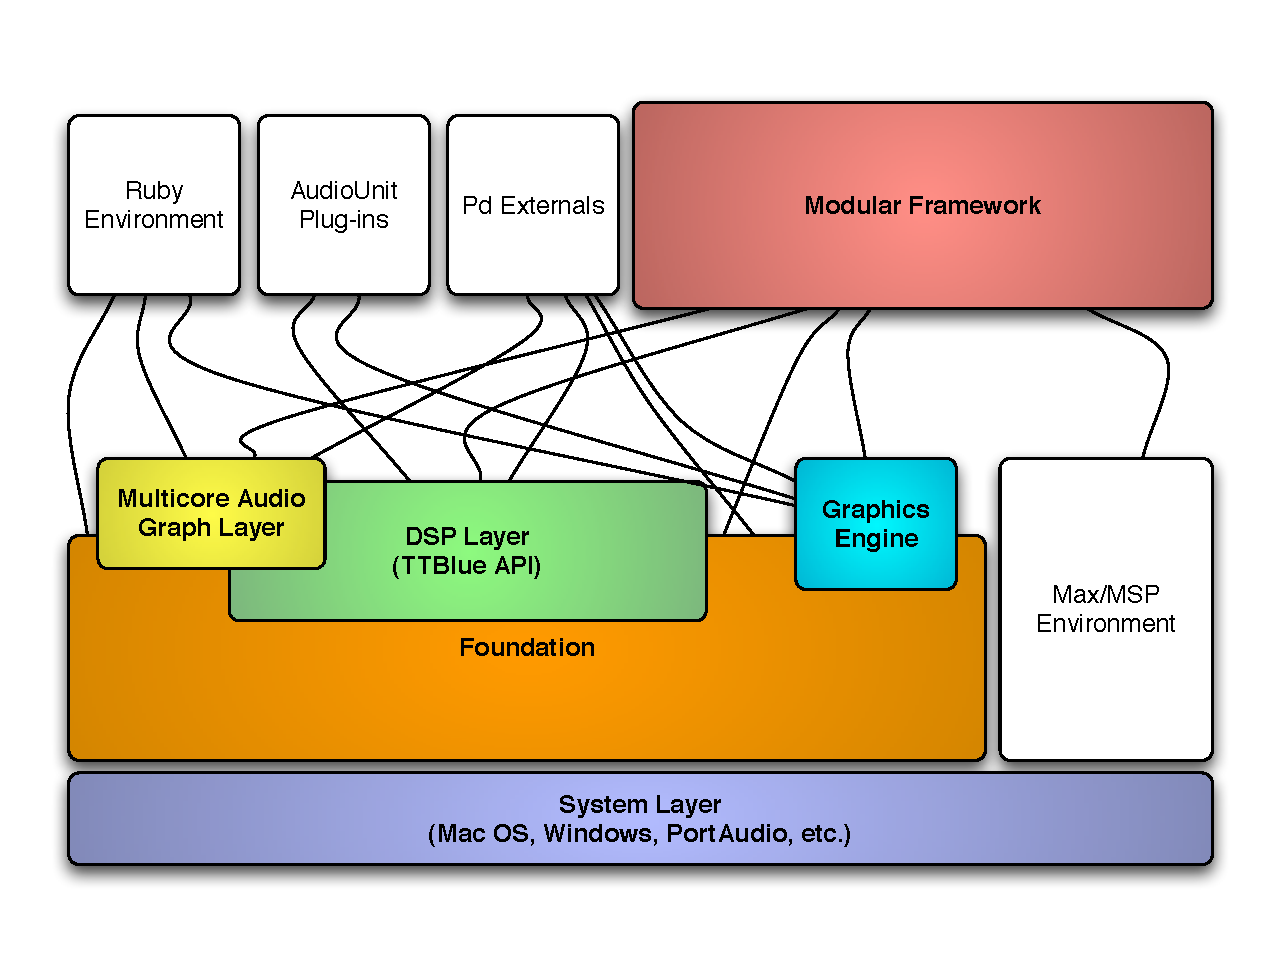
\includegraphics[width=0.9\columnwidth]{layers}}}
\caption{The Jamoma Platform as Layered Architecture.}
\label{fig:layers}
\end{figure}

The Jamoma Platform comprises a number of initiatives working together
(see Figure~\ref{fig:layers}).



\subsection {Frameworks vs. Environments}

%TODO: Look for how Pascal was relating Lloopp and TapeMovie as environments when compared to Jamoma Modular, the same thing applies here...

Jamoma Foundation/DSP is not an environment.  It is a framework that you can use to create an environment, or to extend an existing environment, but it is not itself and environment.  That same can be said of the STK but other examples here, such as Marsyas and CLAM, are really full environments in the same way the ChucK or PureData is an environment.


% (end)


%%%%%%%%%%%%%%%%%%%%%%%%%%%%%%%%%%%%%%%%%%%%%%%%%%%%%%%%%%%%%%%%%%%%%%%%%%%%%%%%%%%%%%%%%%%

\section{Structure / API} % (fold)

\subsection{Design}

%The design of the Jamoma Foundation and DSP Library is informed by the qualities Dieter Rams' ``ten principles for good %design''\footnote{http://www.vitsoe.com/en/gb/about/dieterrams/gooddesign}
%\begin{packed_item}%\begin{itemize}
%	\item Good design is innovative
%	\item Good design makes a product useful
%	\item Good design is aesthetic
%	\item Good design helps us to understand a product
%	\item Good design is unobtrusive
%	\item Good design is honest
%	\item Good design is long-lasting
%	\item Good design is consequent to the last detail
%	\item Good design is concerned with the environment
%	\item Good design is as little design as possible
%\end{packed_item}%\end{itemize}


\subsection{The API}

The basic calls: lifecycle, attributes, messages

\subsubsection{Attributes}

Attributes are not merely maintaining the state of a single value but are multifaceted entities whose behavior is modified through the use of properties\cite{Place:2008params}.


\subsubsection{An Example Class: the DC Blocker?}

Or maybe a FunctionLib thing to show off the calculate method?
% (end)


%%%%%%%%%%%%%%%%%%%%%%%%%%%%%%%%%%%%%%%%%%%%%%%%%%%%%%%%%%%%%%%%%%%%%%%%%%%%%%%%%%%%%%%%%%%

\section{Components} % (fold)

\subsection{The Standard Libraries}

The FilterLib
The EffectsLib
The MathLib
DataspaceLib
FunctionLib 
ChaosLib [NP]
etc.

\subsection{Unit Testing}

baked right in (though currently on a branch that needs to be finished and merged to master...)


\subsection{Serialization}

I had started this code, but where is it now?


\subsection{Ruby Language Bindings}

This is cool!

example: filter design using reflective features in a web browser

MVC
    Model: DSP Objects/Foundation DSP
    View: web browser
    Controller: ruby/rails

MVC
    Model: DSP Objects/Foundation DSP
    View: TTGraphics
    Controller: Max

MVC
    Model: Virage Sequencer \url{http://www.plateforme-virage.org/}
    View: TTGraphics
    Controller: OSC
    
    
Possible models:
    DSP Objects/Foundation DSP
    Virage Sequencer
Possible Controllers:
    Ruby/Rails
    OSC
    Mac
    CopperLAN
Possible Views:
    Max
    TTGraphics
    Web browser


% (end)


%%%%%%%%%%%%%%%%%%%%%%%%%%%%%%%%%%%%%%%%%%%%%%%%%%%%%%%%%%%%%%%%%%%%%%%%%%%%%%%%%%%%%%%%%%%

\section{Examples} % (fold)

1. DC Blocker class
2. How to wrap the class
3. How to combine two classes: e.g. noise + bandpass filter
4. FM that can be repatching the FM unit in real time (different algorithms)  -- (perhaps this could a part of the discussion section?) 
    %TODO: Trond will try to find examples/graphics illustrating this for further discussions between authors
    %TODO: interpolation for TTWavetable
    %TODO: Non-linear filters - limiting or saturation inside the filter as xn is cast to xn-1 and yn to yn-1 (switching the feedback-filter on the fly)

% (end)


%%%%%%%%%%%%%%%%%%%%%%%%%%%%%%%%%%%%%%%%%%%%%%%%%%%%%%%%%%%%%%%%%%%%%%%%%%%%%%%%%%%%%%%%%%%

\section{Discussion / Applications} % (fold)

real-world use includes Electrotap's Tap.Tools\footnote{http://electrotap.com/taptools}, Cycling '74's Hipno\cite{Place:2005}, and the Jamoma Modular Framework\cite{Place:2006}


\subsection{Spatialization}

Spatialization at the Encoding/Decoding and Authoring layers\cite{Peters:2009}.  In fact, through the development of the NodeLib we are now able to work also at the Scene Description Layer by communicating as SpatDIF\cite{Peters:2008spatdif}.

One example that is ready for implementation in the Jamoma DSP library is DBAP\cite{Lossius:2009}.


\subsection{User Interface Development}

Yup yup yup yup...

\subsection{AudioUnit Creation}

Blah blah blah...

\subsection{External Object Generation for Max/MSP and PureData}

Class wrappers...  What about SuperCollider?  I guess we should actually do it first before we claim that we can.

\subsection{Ruby and Ruby on Rails}

Server-side web application framework.  :-)

\subsection{ViMiC}
In the summer of 2009 we combined the application domains of spatialization, graphical rendering, and AudioUnit creation to create a plug-in version of ViMiC\cite{Peters:2008b}.

% TODO: Nils, do you have a a screenshot we could add here?  [tap]

\subsection{Rapid Prototyping Environment}

Because we can put together objects in the environment of our choice: Max, Pd, a DAW if we use AudioUnits, and then even a web-browser using Ruby on Rails.  Then we can move the code from one environment to another easily, or port it back to C++ with minimal effort.

\subsection{Mapping}

Introspection features of the Jamoma Foundation make it possible to query objects to automate the process of creating mappings and advanced control of the objects such as those cataloged in \cite{Pendharkar:2006}.  


% (end)

%%%%%%%%%%%%%%%%%%%%%%%%%%%%%%%%%%%%%%%%%%%%%%%%%%%%%%%%%%%%%%%%%%%%%%%%%%%%%%%%%%%%%%%%%%%

\section{Further Development} % (fold)

\subsection{UI}

Automated UI editor generation through Jamoma Graphics.

\subsection{Multicore}

Not sure what to say here yet -- need to do some assessment on Multicore (fun fun fun).

\subsection{ClassWrappers}

For more environments, such as VST and SuperCollider

\subsection{Standard Library Expansion}

Spectral processing \\

Granular processing   \\

More effects (reverb, pitch-shifting, chorus) 


Spectral(FFT) Processes\\

SynthesisLib

\subsection{Scheduler}

Initial work on a scheduler for the DSP library was begun in 2007.  Competing priorities have left it unfinished...  More interesting models for scheduling, such as the the model implemented in ChucK provide impetus for further research into new approaches to this topic.

\subsection{Tools}

- Unit testing      \\

- Integrated Analysis and Benchmarking -- perhaps reference the upchuck operator in ChucK?
   -- This integrated analysis and benchmarking could also provide the basis by which an audio graph such as Jamoma Multicore is able to evaluate how to optimize the processes in the graph to make intelligent decisions on how to distribute the processing among threads or processors.


\subsection{Web Browser Support}
We have begun implementing support for server-side integration of the Jamoma Runtime via the Ruby language bindings and Ruby on Rails\footnote{http://rubyonrails.org}.  To fully leverage the DSP library and Jamoma Foundation in a web-browser we need the ability to invoke the runtime on the client-side of the equation through a web browser plug-in similar to that done in the iARS Project\cite{Frauenberger:2003}.

\subsection{NodeLib}

As a means of addressing parts of the system via OSC.  Somewhat like what Marsyas does.  An implementation of the ideas presented in\cite{Place:2008osc}.

\subsection{Processing Arrays}
[12/10/09 7:58:39 PM] Nils Peters: on the other hand, IMHO in most use cases you want to have separate control over the filter parameter of each channel
[12/10/09 8:00:26 PM] Nils Peters: or the delay
[12/10/09 8:00:41 PM] Nils Peters: You want to set different delays to your input channels

[12/10/09 7:59:32 PM] Tim Place: It could be possible to create an object which wraps an array of objects that process each channel individually
[12/10/09 7:59:58 PM] Tim Place: I think that would address the filter problem you mention more generally


\subsection{Figures, Tables and Captions}

\begin{table}[htbp]
\begin{center}
\begin{tabular}{|l|l|}
\hline
String value & Numeric value \\
\hline
hello ICMC  & 1073 \\
\hline
\end{tabular}
\end{center}
\caption{Table captions are placed below the table.}
\label{tab:example}
\end{table}


% (end)

%%%%%%%%%%%%%%%%%%%%%%%%%%%%%%%%%%%%%%%%%%%%%%%%%%%%%%%%%%%%%%%%%%%%%%%%%%%%%%%%%%%%%%%%%%%

\section{Summary} % (fold)

Jamoma Foundation and DSP provide a flexible, user-extendable, runtime environment for creating and using audio and digital signal processing objects.  Due to its advanced use of dynamic binding and message-passing paradigm, the building blocks can be reconfigured at runtime without requiring re-compilation, but with the unit generators themselves compiled as C++ and performing block-processing we retain the performance of a compiled language.


"A well-defined API can also speed up the development process, since the implementation can focus more on the algorithmic aspects and less on implementation issues like API design." \cite{Lerch:2005}

The power of this runtime is demonstrated through the ability to compile objects for Max, Pd, AudioUnits, VST, etc.  The future includes Multicore.




% (end)

%%%%%%%%%%%%%%%%%%%%%%%%%%%%%%%%%%%%%%%%%%%%%%%%%%%%%%%%%%%%%%%%%%%%%%%%%%%%%%%%%%%%%%%%%%%

\section{Acknowledgements} % (fold)

Dave Watson, Joshua Kit Clayton, Théo Delahogue, Tristan Mathews

% (end)

%%%%%%%%%%%%%%%%%%%%%%%%%%%%%%%%%%%%%%%%%%%%%%%%%%%%%%%%%%%%%%%%%%%%%%%%%%%%%%%%%%%%%%%%%%%

\bibliographystyle{IEEEtranS}
\bibliography{../../Shared/bibtex/Jamoma} % requires file template.bib

\end{document}
